%% The following is a directive for TeXShop to indicate the main file
%%!TEX root = diss.tex

\chapter{Related Work}
\label{ch:RelatedWork}

\begin{epigraph}
    \emph{
       The computing scientist’s main challenge is not to get confused by the 
       complexities of his own making.
     } ---~Edsger W. Dijkstra
\end{epigraph}

\noindent Researchers have investigated both the questions that developers ask 
as they understand and evolve their systems, and the efficacy of tools 
that support developers in answering their questions during software change 
tasks.

\par Developers find it challenging to understand code in modern codebases for
a number of reasons.
Many codebases today are large and complex, with some meeting the definition of 
an \emph{ultra-large-scale system} \cite{feiler-2006-ulss}.

\par Google reported in 2016 that its monolithic software codebase was composed
of approximately 1 billion files, with a history of 35 million commits in a
repository that contains 85 terabytes of data and 2 billion lines of code
\cite{potvin-2016-google}.
Of course, not all software systems in existence today are quite comparable in 
scale, but Google's codebase helps to contextualize the challenges that 
developers may face in understanding the systems they wrangle each day.
The size, complexity, and indirection that is becoming commonplace in systems
today \cite{latoza-2010-reach} are pushing the already-elusive goal of
enabling developers to more easily enderstand their code into new and 
uncharted territories.

\section{Questions that Developers Ask}
\label{sec:QuestionsThatDeveloperAsk}

\noindent Developers have a large number of information needs that must be
addressed during their day-to-day workflows.
These information needs often present themselves as a variety of questions
that require the integration of often-disparate sources of information
\cite{fritz-2010-info-frag}.
For example, to understand how a defect was introduced, a developer may have to
read the source code of a program, find additional context within a bug report
or a project tracker, or resort to speaking to other developers who may have 
more information. 

\par Other questions that developers may ask are more focused, and may involve
querying only one source of information, such as a single program or a
collection of modules in a system.
As developers work to evolve and understand specific parts of their systems,
they may ask: ``where are instances of this class created?" or
``what data can we access from this object?" as they try to discover entities
and relationships in object-oriented systems
\cite{sillito-2006-questions-during-task}.
Additional questions that developers may ask are related to 
the control-flow or the data-flow through a program, such as 
``why isn't control reaching this point in code?" and 
``what parts of this data structure are being accessed in this code?" 
\cite{sillito-2006-questions-during-task}.

\subsection{Reachability Questions}
\label{subsec:ReachabilityQuestions}

\par Researchers have conducted studies that investigate both the 
frequency and difficulty of answering some of the focused questions that 
developers ask during change tasks.
LaToza et al. found that a significant portion of a developer's work involves 
answering reachability questions.
A reachability question is a search across feasible paths through a program for 
target statements matching search criteria \cite{latoza-2010-reach}.
In a survey distributed to 2000 developers employed at Microsoft's Redmond
campus, 460 developers reported asking questions that could be phrased as 
reachability questions more than 9 times a day.
Of the developers who responded, 82\% of them rated one or more of the
reachability questions as at least somewhat hard to answer.
\cite{latoza-2010-reach}.
Not only are reachability questions difficult to answer, but the process of
investigating them is also time-consuming.
A field study of 17 developers found that of the 10 longest activities
undertaken by developers, 9 were associated with reachability questions
\cite{latoza-2010-reach}.

\noindent LaToza et al. formalized two types of reachability questions, named
\textit{find} and \textit{compare} \cite{latoza-2010-reach}.
A \textit{find} question is of the form \findq{}; where \textit{SC} and
\textit{TR} are variable parameters.
\textit{TR} represents a set of concrete program traces, where each trace 
\textit{tr} is a list of tuples $\langle s, env \rangle$. 
In each tuple, $s$ is a statement, and $env$ maps each variable in $s$ to a
value.
\textit{SC} represents search criteria that acts a a function that prunes the
set of traces \textit{TR} to a subset that is relevant to the reachability
question being asked.
As an example of a \textit{find} question, a developer may ask: ``where does
the string \bsq{error} come up in the control-flow of this method called 
\texttt{openConnection}?"
To formalize this into a \textit{find} question, we define \textit{SC} as
$grep(`error\textrm')$, and \textit{TR} as 
$trace(p, \ m_{start}, \ m_{end}, \ C)$, where $p$ is the entire program under
inspection, $m_{start}$ and $m_{end}$ represent the start and end of the
control-flow of the method \texttt{openConnection}, and $C$ is a filtering
constraint that is left unspecified.
The resulting formalization is:
\begin{align*}
  find \ grep(`error\textrm') \ in \ trace(p, \ m_{start}, \ m_{end}, \ C)
\end{align*}
The result of this formalization is a a set of traces that contain statements
where the string \bsq{error} occurs, which a developer may use to help answer
their orignal question.

\par A \textit{compare} question requires the analysis of two concrete traces, 
and is of the form \compareq{}. 
First, an attempt is made to match each trace $tr_a \in TR_a$ to a trace 
$tr_b \in TR_b$.
The result of this operation may be represented as a list of tuples 
$\langle tr_a, tr_b \rangle$.
For each tuple in the resulting list, \textit{compare} attempts to match 
$\langle s_a, env_a\rangle \in tr_a$ to $\langle s_b, env_b \rangle \in tr_b$.
Each matching tuple is coalesced into traces $tr_{common}$, that form one
of the outputs of the \textit{compare} question: $TR_{common}$.
The tuples in $tr_a$ and $tr_b$ for which no match is found are collected into
the outputs $TR_1$ and $TR_2$.
A developer may ask a \textit{compare} question as they refactor code.
``Is this code correct?" \cite{latoza-2010-hard-questions} is a common
question that is often asked.
Assuming ``correct" in the context of refactoring to mean that there are no
functional changes to business logic, the resulting formalization of the
previous question might be:
\begin{align*}
  compare(TR_{pre}, \ TR_{post})
\end{align*}
Where $TR_{pre}$ is the set of traces from the program prior to the refactor,
while $TR_{post}$ is the set of traces from the program after the refactor.
Using $TR_{pre}$ as a ground truth, the developer might inspect the ouputs
of the formalization: $T_{common}, T_1,$ and $T_2$, and draw conclusions
regarding the correctness of the refactor.

\section{Answering Reachability Questions}
\label{sec:AnsweringReachabilityQuestions}

\acp{IDE} such as IntelliJ IDEA and Visual Studio include tools that developers 
might adopt in answering reachability questions, even if they were not designed
for that purpose.
For example, a developer might generate a call graph for a set of methods in a
class, and manually traverse it to trace or collect items of interest.
Although a number of built-in tools could be adopted in helping developers
answer reachability questions, it is also suggested that developers could 
perform coding tasks more quickly and accurately with tools that more directly 
support answering reachability questions \cite{latoza-2010-reach}.

\subsection{Low-level Support for Reachability Questions}
\label{subsec:LowLevelSupportReachabilityQuestions}

A common reachability question that developers might ask is: ``where does this
value come from?"
To answer this type of question, a developer could invoke a general-purpose
slicing mechanism (Figure \ref{fig:IntelliJDataflow}) that produces  a set of 
data-flow traces (Figure \ref{fig:IntelliJDataflowResult}).

\par Although the information produced by mechanisms such as general-purpose
slicing and data-flow analysis may be complete and useful, 

% TODO: blah blah they may not be usable/intuitive etc...

\begin{figure}[ht]
\centering
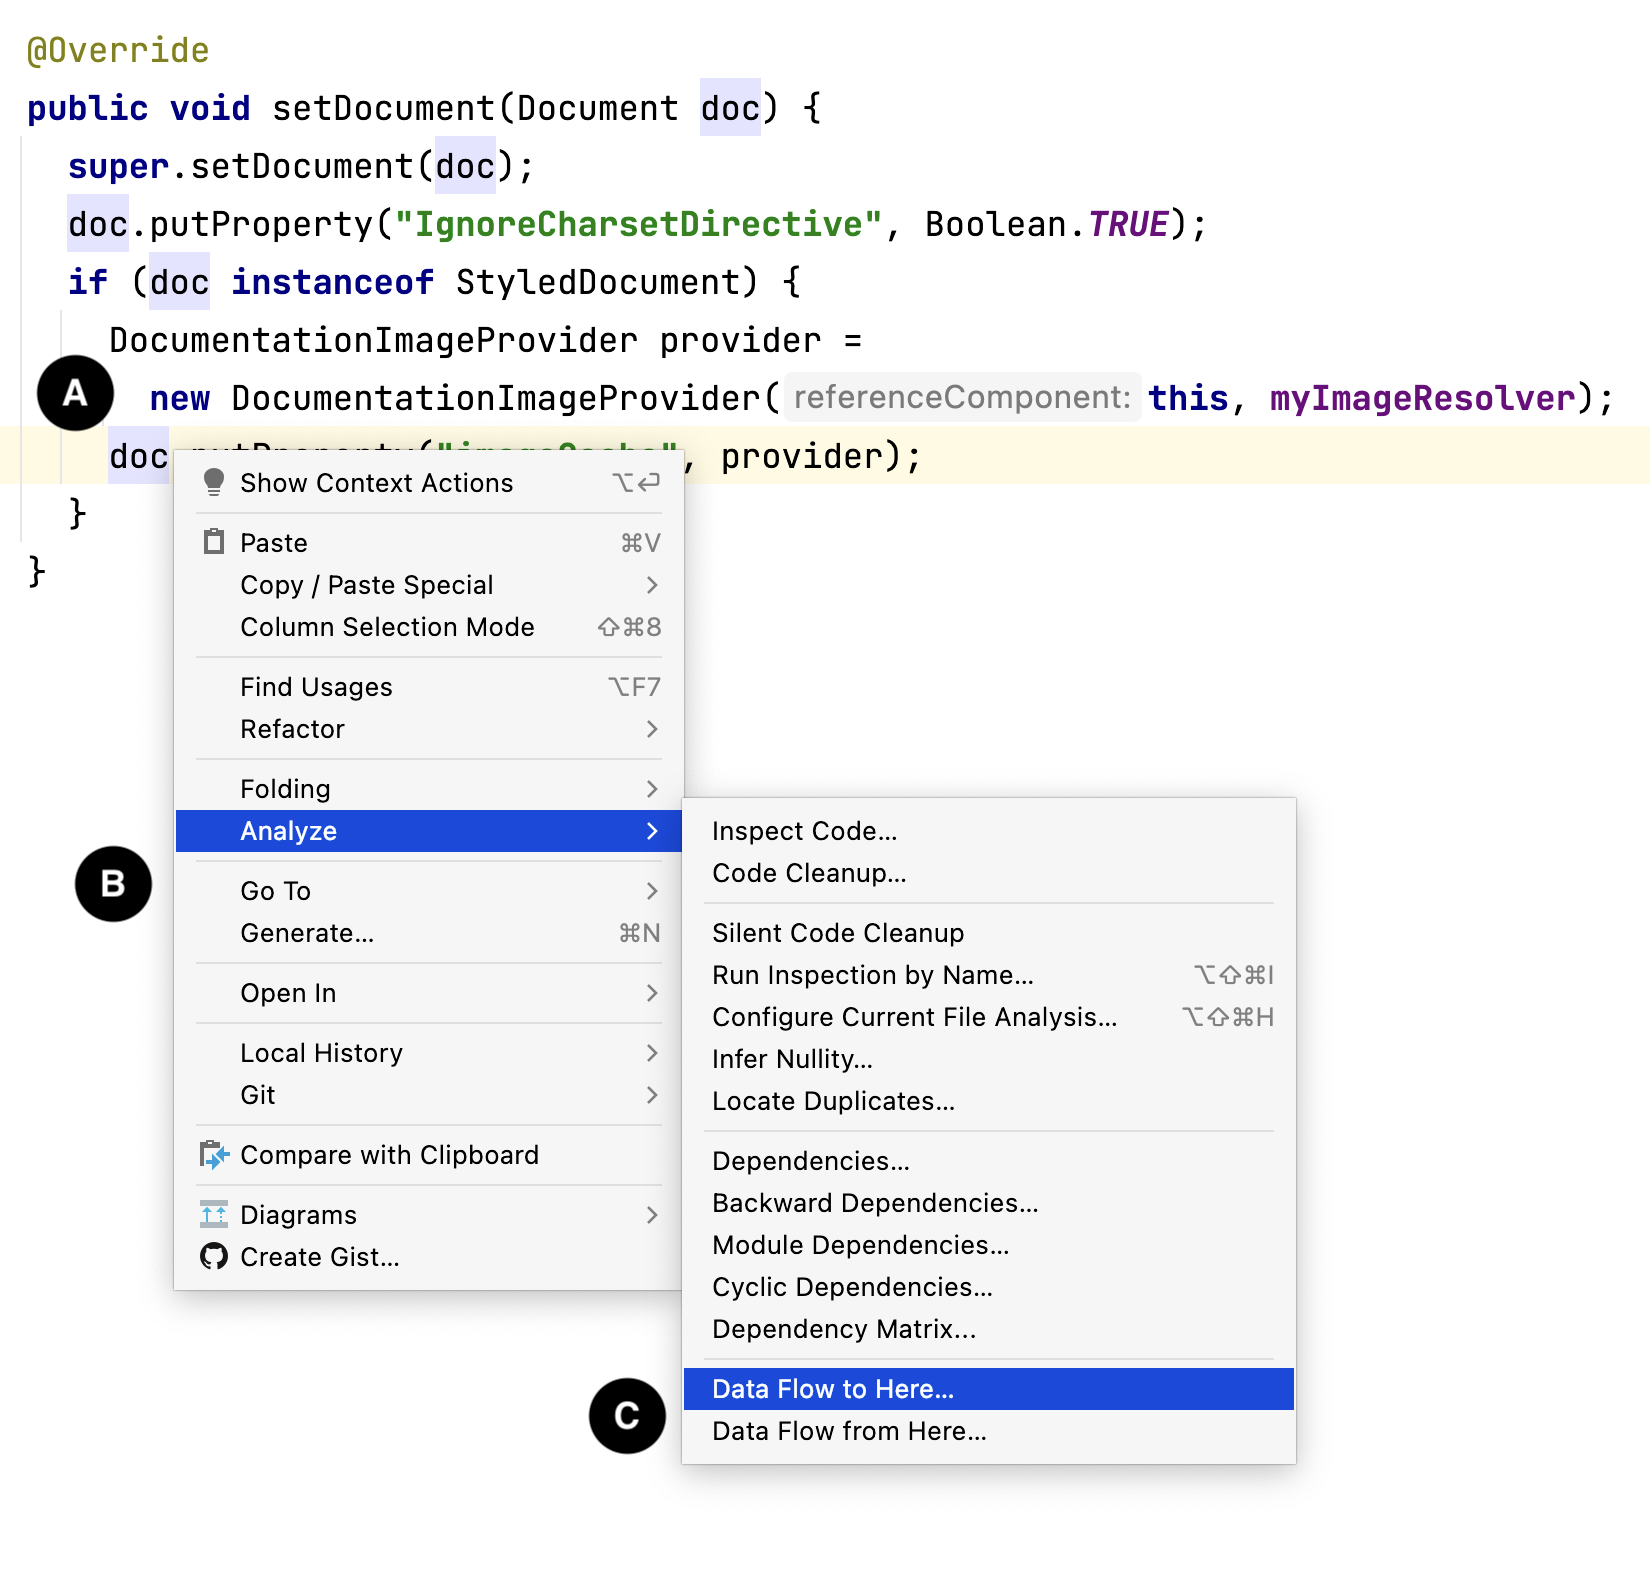
\includegraphics[width=\textwidth]{./figs/intellij-dataflow.png}
\caption{
  A data-flow analysis workflow in IntelliJ IDEA. (A) is the value of
  interest, \texttt{doc}. (B) exposes the variety of analyses that are
  available to developers for \texttt{doc}. (C) invokes a data-flow analysis
  of values that flow into \texttt{doc}.
}
\label{fig:IntelliJDataflow}
\end{figure}

\begin{figure}[ht]
\centering
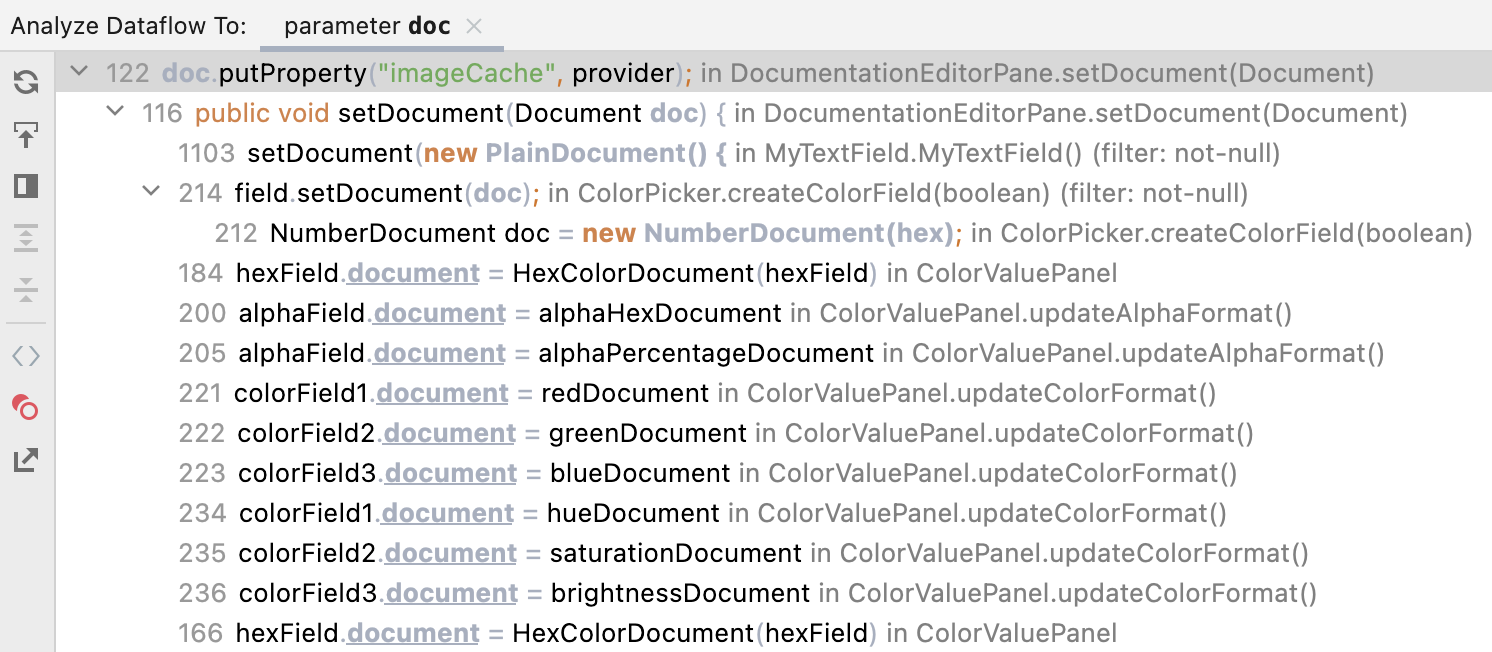
\includegraphics[width=\textwidth]{./figs/intellij-dataflow-result.png}
\caption{
  The output of invoking a ``Dataflow to here..." analysis on \texttt{doc}
  (Figure \ref{fig:IntelliJDataflow}). Each line represents an assignment
  operation to \texttt{doc}. Information such as the line of code, and 
  enclosing method are displayed.
}
\label{fig:IntelliJDataflowResult}
\end{figure}
% TODO: this isn't a question that requires specialized/high-level support

\section{Tools that Support Reachability Questions}
\label{sec:ToolsSupportReachabilityQuestions}

\noindent Tools today employ both dynamic and static approaches to gathering
program information for developers.
The Whyline analyzes runtime information gathered from an offline dynamic
analysis of an execution trace to generate a set of question and answer pairs
that are presented to developers \cite{ko-2004-whyline}.
GetMeHere developed at Microsoft Research leverages static analysis by
translating high-level developer questions into low-level program verification 
problems that are dispatched to an \ac{SMT} solver \cite{barnett-2014-get}, 
removing the need for developers to run their programs to analyze them.

\subsection{The Whyline}
\label{subsec:TheWhyline}

\par The Whyline was initially developed as an interogative debugging interface
for the Alice programming language. Later, the Java Whyline was developed to 
support the Java programming language and the needs of professional developers.
At a high-level, the Whyline enables developers to select questions about a
program's output, and it then helps developers to work back from from the 
selected output to its causes \cite{ko-2009-java-whyline}.
These questions are phrased as ``why did" and ``why didn't"
queries about program output.
For example, consider a case when a variable \texttt{foo} is being erroneously 
set to some value \texttt{v}.
A developer could choose to investigate the cause of this erroneous program
behaviour by running the program, opening the Whyline window and selecting
``why did \texttt{foo} $=$ \texttt{v}?" and a \emph{temporal context}, which is
a specified time-frame that they wish to investigate.
The Whyline then presents a view of all statments of the program within the
temporal context that contributed to the line where \texttt{foo} has the value
\texttt{x}. 
The Whyline's approach of presenting a pre-defined subset of questions about the 
output of programs has benfits, as it avoids speculation about the causes of
a failure, and simplifies the exploration of code responsible for the output
\cite{ko-2009-java-whyline}.
An experiment was conducted to evaluate the efficacy of the Whyline on 
isolating the causes of two bug reports from an open source project.
It was found that the Whyline users were successful about three times as often
and about twice as fast compared to the control group who used conventional
debugging tools and techniques.

\par Although the Whyline was designed as a stand-alone tool, it presents an 
interface to a developer that resembles those of commonly used \acp{IDE} such
as Microsoft Visual Studio, IntelliJ IDEA, and Eclipse.
Figure \ref{fig:WhylineQuestion} shows the Whyline interface as it is used
to investigate the output of a \ac{GUI} application.
Developers are able to choose a question from the dropdown menu that appears
next to some observable program output.
The Whyline then presents a view that traces the execution of the program
to the specific lines that have an effect on the output under investigation.
This view is presented in Figure \ref{fig:WhylineTrace},
where an editor-like view shows two lines of code in different source files
that affect program output.

\begin{figure}[ht]
\centering
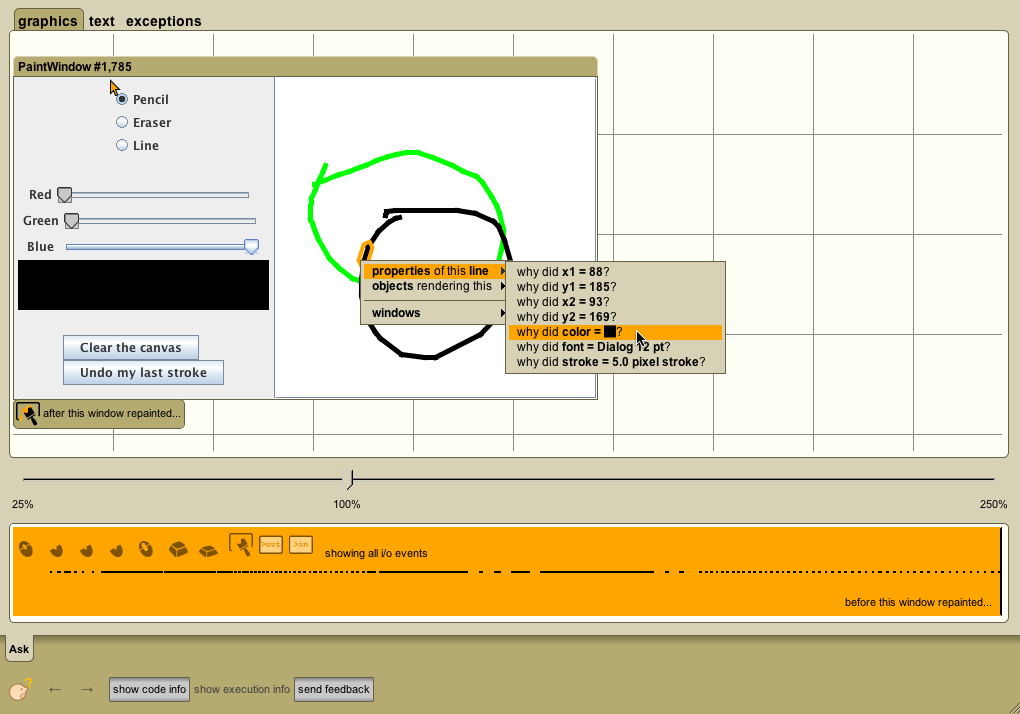
\includegraphics[width=\textwidth]{./figs/whyline-question-interface.png}
\caption{The interrogative debugging interface presented by Whyline.}
\label{fig:WhylineQuestion}
\end{figure}

\begin{figure}[ht]
\centering
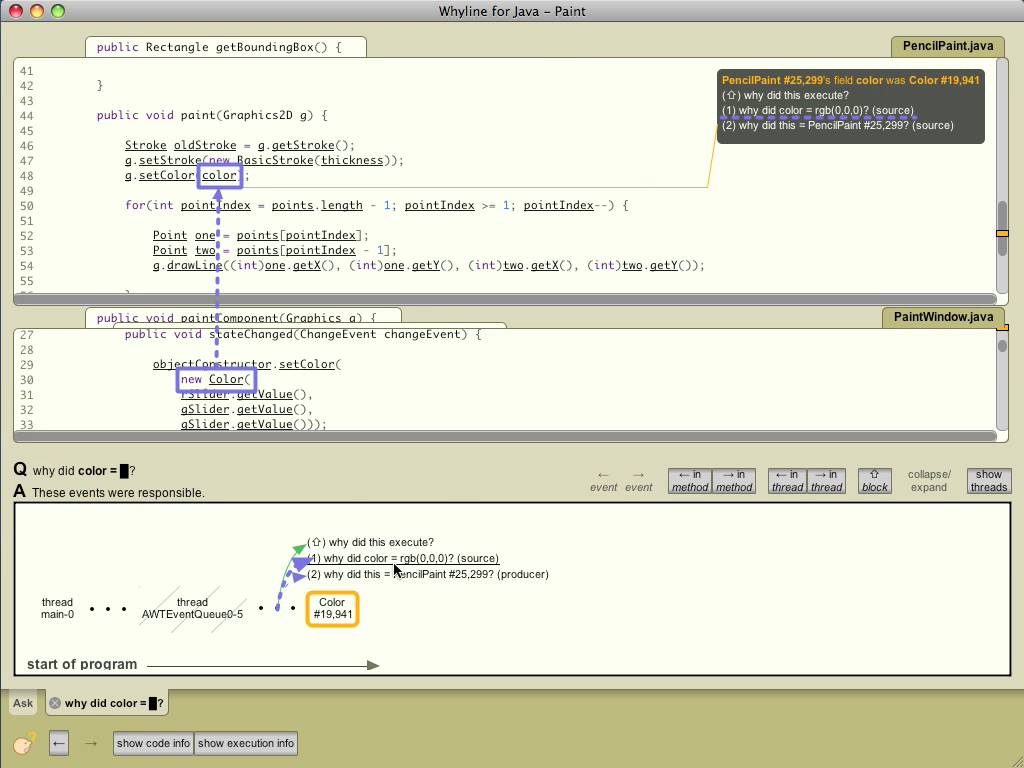
\includegraphics[width=\textwidth]{./figs/whyline-trace-back.png}
\caption{The high-level program trace presented by Whyline.}
\label{fig:WhylineTrace}
\end{figure}

\subsection{GetMeHere}
\label{subsec:GetMeHere}

\par Similar to the Whyline, GetMeHere enables developers to select a line of 
code as a point of interest and visualize the execution that reaches the given 
point.
Where it differs, however, is in how it is able to generate this execution
by using an SMT-based static analysis \cite{barnett-2014-get} without having to
execute the code.
GetMeHere is also presented as a general query engine, where developers can
specify a slice in a program, and execute queries that represent reachability
questions over the given slice \cite{barnett-2014-get}.
The flexibility afforded by GetMeHere enables to developers to fine-tune their
queries, but may introduce some of the speculation about program failures or
erroneous behaviour that the Whyline attempts to minimize.
GetMeHere was evaluated on three benchmark programs, all written in C\#.
The sizes of the benchmark programs ranged from 650 to $11,000$ lines of code,
which is relatively small by modern standards.

\par Unlike the Whyline, GetMeHere was built as an extension to the Visual
Studio \ac{IDE}, and not as a standalone application.
GetMeHere displays an execution trace using the Microsoft Debugger Canvas 
\cite{bragdon-2012-canvas}, an industrial implementation of the earlier 
Code Bubbles \cite{bragdon-2010-code-bubbles} paradigm for Visual Studio
\cite{barnett-2014-get}.

\section{How Developers Use Tools to Understand Programs}
\label{sec:HowDevelopersUseToolsToUnderstandPrograms}

\noindent In practice, developers still face difficulties in finding answers 
for their questions during development tasks, even with the tooling available 
to them.
This appears to be in part due to the inevitability of imperfect mappings from
high-level developer questions to the low-level analysis facilities afforded
by prograam comprehension tools.
In fact, a study of industrial programmers [sic] by Sillito et al. showed that 
participants often struggled to refine and map their questions to tools
that could be used to answer them \cite{sillito-2006-questions-during-task}.

\par The usability of software engineering tools may also be a significant
factor on how developers use tools to help answer their questions.
Many software tool developers rely on their own intuition for how a tool should
work, eschewing established criteria and procedures for evaluating their 
usability \cite{toleman-98-soft-tools}.
Consequently, the tools available to developers today may be useful, but
ultimately be lacking in terms of their usability.
This lack of usability may even force developers to explore alternative
strategies in understanding and evolving their systems.
In a study of 28 developers from a wide range of companies of different sizes,
Roehm et al. found that 14 of them effectively cloned code due to the
difficulty of understanding the existing code and the consequences of their
changes \cite{roehm-2012-comprehend-software}.
Developers may also choose to abandon the use of purpose-built program
comprehension tools altogether.
In the same study conducted by Roehm et al., 22 deveopers used an IDE
for development and comprehension tasks.
However, none were observed making use of the IDE's built-in program 
comprehension features, such as visualization and concept localization
\cite{roehm-2012-comprehend-software}.

\par Developers spend a significant portion of the day attempting to answer
questions about their code.
Although there are specialized tools that exist to aid developers in this task,
they are not without their limitations. 
The Whyline represents a promising approach in enabling developers to answer 
questions about the runtime behaviour of their code.
However, it only enables a retrospective analysis of a program, and does not 
support on-the-fly queries.
GetMeHere attempts to bypass the need for an execution trace and provide support
for on-demand queries by translating high-level developer questions into SMT
instances. 
Although the results presented by Barnett et al. are promising, the
relatively small size of the systems GetMeHere was evaluated on leaves more to
be investigated about the scalability of their approach.

\endinput

TODO: add a paragraph about what my thesis attempts to contribute (in relation
to the related work section).

